\documentclass{article}
\usepackage[utf8]{inputenc}
\usepackage[margin=0.5in]{geometry}
\usepackage{amsfonts}
\usepackage{setspace}
\usepackage{graphicx}

\title{Assignment 4, Design Specification}

\author{Abhiraj Gogia \\\\ COMPSCI 2ME3 }
\date{\today}

\begin{document}
\doublespacing

\maketitle

This Module Interface Specification (MIS) document contains modules, types and methods for implementing the game \textit{2048}. At the start of each game, begins with a $4 \times 4$ grid of squares, sparsely filled with numbers. The player can then shift all the numbered squares in the grid to the right, left, upward, or downward. If numbers of the same value collide, they combine to form a larger number. After each move made by the player, new numbers will randomly spawn on the grid. The game ends when the player can no longer make any moves which change the position of the board (i.e. every block is stuck in place, as none of them can combine). The game will always terminate, but it's the player's job to last as long as they can and achieve the highest possible score. Throughout this specification document, the grid of squares may be referred to as a matrix or board interchangeably. Furthermore, an empty square on the board will be one that holds a value of zero. In addition to this, the row number of the grid increases when going from top to bottom, and the column number of the grid increases when going from left to right. The game uses a graphic user interface (GUI), therefore, it cannot simply be run in terminal on Mills. Thus, to run the game, run the 'Main` Module from your integrated development environment (IDE).

\section*{Overview of the design}
This design applies a variation of the Model-View-Controller (MVC) design pattern where the controller is integrated into the View Module. The MVC design pattern was implemented in the following way:  the module \textit{BoardStatus} stores the state of the board and takes care of any manipulation of the board elements. An ASCII \textit{Viewer} module displays the state of the board in terminal. A Viewer/Controller Module by the name of \textit{InputReader}, records and processes user input and displays it on a GUI.

\subsection*{Likely Changes my design considers:}
\begin{itemize}
    \item Adjustable UI to allow for varying colour modes.
    \item Room for adding addition inputs that execute actions (like a mouse click or other key inputs).
\end{itemize}
\newpage

\section*{Board State ADT Module}
\subsection*{Template Module}
BoardStatus
\subsection*{Uses}
InputReader, Random
\subsection*{Syntax}
\subsubsection*{Exported Constants}
None
\subsubsection*{Exported Access Programs}
\begin{tabular}{ | c | c | c | c | }
        \hline 
    
          \textbf{Routine name} & \textbf{In} & \textbf{Out} & \textbf{Exceptions}\\
          \hline 
          getBoardValues & & Integer[ ][ ] & \\\hline
          verticalCombine & $\mathbb{N} \times \mathbb{N}\times \mathbb{N}$ & & \\ \hline
          horizontalCombine & $\mathbb{N} \times \mathbb{N}\times \mathbb{N}$ & & \\ \hline
          shiftRight & & & \\ \hline
          shiftLeft & & & \\ \hline
          shiftUp & & & \\ \hline
          shiftDown & & & \\ \hline
          newElement & & & \\ \hline
          increaseScore & \mathbb{N} & & \\ \hline
          
\end{tabular}

\subsection*{Semantics}
\subsubsection*{State Variables}
boardValues : sequence of sequence of $\mathbb{N}$  \\
score : $\mathbb{N}$ 

\subsubsection*{State Invariant}
None

\subsubsection*{Assumptions}
\begin{itemize}
    \item None
\end{itemize}

\subsubsection*{Access Routine Semantics}
BoardStatus():
\begin{itemize}
    \item transition: boardValues $:= \langle i :$ Integer $ | i \in \;$boardValues$\; : 0 \rangle$
    \\ boardValues$[i][j] := 2$ \\
    boardValues$[k][l] := 2$ \\\# Where $i, j, k, l$ are random integers between $0$ and $3$ using the nextInt() function in the Random module and $\neg(i \equiv k \land j \equiv l)$
    \item output: \textit{out $:=$ self}
    \item exception: None
\end{itemize}
getBoardValues():
\begin{itemize}
    \item output: \textit{out $:=$ boardValues}
    \item exception: none
\end{itemize}
verticalCombine(\textit{index1, index2, column}):
\begin{itemize}
    \item transition: $\langle$ boardValues$[$index1$][$column$] \equiv $ boardValue$s[$index2$][$column$] \Rightarrow$ boardValues$[$index1$][$column$] := 0 \\ \land$ boardValue$s[$index2$][$column$] :=$ boardValue$s[$index2$][$column$] \times 2 \; \land \;$ increaseScore(boardValue$s[$index2$][$column$] \times 2$) $\land$ inputReader.setText(``2048 $|$ Score: " +  BoardStatus.getScore()) $|$ boardValues$[$index1$][$column$] \neq 0$ $\land $ \\ boardValue$s[$index2$][$column$] \equiv 0 \Rightarrow$ boardValues$[$index2$][$column$]$ $:= $boardValues$[$index1$][$column$]\; \\ \land$ boardValues$[$index1$][$column$] := 0 \rangle$
    \item exception: none
\end{itemize}
horizontalCombine(\textit{index1, index2, row}):
\begin{itemize}
    \item transition: $\langle$ boardValues$[$row$][$index1$] \equiv $ boardValue$s[$row$][$index2$] \Rightarrow$ boardValues$[$row$][$index1$] := 0 \\ \land$ boardValue$s[$row$][$index2$] :=$ boardValue$s[$row$][$index2$] \times 2 \; \land \;$ increaseScore(boardValue$s[$row$][$index2$] \times 2$) $\land$ \\ inputReader.setText(``2048 $|$ Score: " +  BoardStatus.getScore()) $|$ boardValues$[$row$][$index1$] \neq 0$ $\land $ \\ boardValue$s[$row$][$index2$] \equiv 0 \Rightarrow$ boardValues$[$row$][$index2$]$ $:= $boardValues$[$row$][$index1$]\; \land$ boardValues$[$row$][$index1$] := 0 \rangle$
    \item output : none
    \item exception: none
\end{itemize}
shiftRight():
\begin{itemize}
    \item transition: $\langle i :$ Integer $ |\; i \in [0..3] : \langle j : $ Integer $ |\; j \in [0..2]: $ horizontalCombine$(j, j + 1, i) \rangle \rangle \; \land \;$ newElement()
    \item output: None
    \item exception: None
\end{itemize}
shiftLeft():
\begin{itemize}
    \item transition: $\langle i :$ Integer $ |\; i \in [0..3] : \langle j : $ Integer $ |\; j \in [2..0]: $ horizontalCombine$(j, j - 1, i) \rangle \rangle \; \land \;$ newElement()
    \item output: None
    \item exception: None
\end{itemize}
shiftDown():
\begin{itemize}
    \item transition: $\langle i :$ Integer $ |\; i \in [0..3] : \langle j : $ Integer $ |\; j \in [0..2]: $ verticalCombine$(j, j + 1, i) \rangle \rangle \; \land \;$ newElement()
    \item output: None
    \item exception: None
\end{itemize}
shiftUp():
\begin{itemize}
    \item transition: $\langle i :$ Integer $ |\; i \in [0..3] : \langle j : $ Integer $ |\; j \in [2..0]: $ verticalCombine$(j, j - 1, i) \rangle \rangle \; \land \;$ newElement()
    \item output: None
    \item exception: None
\end{itemize}
boardFull():
\begin{itemize}
    \item output $:= \langle i :$ Integer $ |\; i \in [0..3] : j : $ Integer $ |\; j \in [0..3]: $ boardValue$[i][j] \equiv 0 | \Rightarrow False \;| \; True\rangle$
    \item exception: None
\end{itemize}
newElement():
\begin{itemize}
    \item transition $:= \langle boardFull() \Rightarrow \langle i :$ Integer $ |\; i \in [0..3] : \langle j : $ Integer $ |\; j \in [0..2]: $ boardValues$[i][j] \equiv $ boardValues$[i][j +1] \lor $ boardValues$[j][i] \equiv $ boardValues$[j+1][i] \Rightarrow$ break $|$ inputReader.setText(``2048 $|$ Score: " +  BoardStatus.getScore() + `` $|$ Game Over")$ \rangle \rangle \; |$ boardValues$[i][j] := k$ $\#$ where $i,j$ are random integers between $0 and 4$ selected by Random.nextInt(), where the value of boardValues$[i][j] \equiv 0$, and is set to $k$, which is a random integer $2$ or $4$ that is also selected by Random.nextInt(). This has a $90\%$ chance of being a $2$ and a $10\%$ chance of being a 4. $ \; \rangle$
\end{itemize}
increaseScore(\textit{value}):
\begin{itemize}
    \item transition: score $:= $ score $+$ \textit{value}
    \item out: None
    \item exception: None
\end{itemize}

\subsubsection*{Local Function:}
\begin{itemize}
    

\item setBoardValues: seq of seq of Integers $\rightarrow$ void \\
setBoardValues(\textit{values}): boardValues $:=$ values \\
\item setCell: Integer $\times$ Integer $\times$ Integer $\rightarrow$ void \\
setCell(\textit{value, rowIndex, columnIndex}) : boardValues[\textit{rowIndex}][\textit{columnIndex}] $:= $ \textit{value} \\
\item setScore: Integer $\rightarrow$ void \\
setScore(\textit{values}): score $:=$ values \\

\end{itemize}
\newpage
\section*{ASCII Viewer Module}
\subsection*{Module}
Viewer
\subsection*{Uses}
BoardStatus

\subsection*{Syntax}
\subsubsection*{Exported Constants}
None
\subsubsection*{Exported Access Programs}
\begin{tabular}{ | c | c | c | c | }
        \hline 
    
          \textbf{Routine name} & \textbf{In} & \textbf{Out} & \textbf{Exceptions}\\
          \hline 
          updateValues & &  & \\\hline
          printBoard & & & \\ \hline
          
         
\end{tabular}

\subsection*{Semantics}
\subsubsection*{State Variables}
values : sequence of sequence of \mathbb{N}
\subsubsection*{State Invariant}
None
\subsubsection*{Assumptions}
\begin{itemize}
    \item None
\end{itemize}

\subsubsection*{Access Routine Semantics}
Viewer():
\begin{itemize}
    \item transition : values $:=$ BoardStatus.getBoardValues()
    \item output $:=$ self
    \item exception: None
\end{itemize}
updateValues():
\begin{itemize}
    \item transition: values $:=$ BoardStatus.getBoardValues()
\end{itemize}
printBoard():
\begin{itemize}
    \item out: $\langle i :$ Integer $ |\; i \in [0..3] : \langle j : $ Integer $ |\; j \in [0..3]: $ print(values$[i][j]$ + `` " ) $\rangle$ print(new line) $\rangle$
\end{itemize}

\newpage
\section*{GUI Viewer and Controller Module}
\subsection*{Module}
InputReader
\subsection*{Uses}
BoardStatus

\subsection*{Syntax}
\subsubsection*{Exported Constants}
None
\subsubsection*{Exported Access Programs}
\begin{tabular}{ | c | c | c | c | }
        \hline 
    
          \textbf{Routine name} & \textbf{In} & \textbf{Out} & \textbf{Exceptions}\\
          \hline 
          normalize &$\mathbb{N}$ & $\mathbb{N}$ & \\\hline
          fontChoose & $\mathbb{N}$ & Colour & \\ \hline
          colourChoose & $\mathbb{N}$ & Colour & \\ \hline
          setText & String &  & \\ \hline
          setVal & $\mathbb{N} \times \mathbb{N} \times \mathbb{N}$&  & \\ \hline
          
          
         
\end{tabular}
\subsection*{Semantics}
\subsection*{Environment Variables}
\textit{frame}: A portion of computer screen to display the game. \\
\textit{table} : A portion of the frame that holds and displays data from BoardStatus. \\
\textit{itemLabel} : A label at the bottom of the frame, which is used to display score and messages. \\



\subsubsection*{State Variables}
size : \mathbb{N} \\
data : sequence of sequence of \mathbb{N}

\subsubsection*{Assumptions}
\begin{itemize}
    \item Assumes that GUI will be run after a BoardStatus() ADT is initialized.
\end{itemize}
\subsubsection*{Access Routine Semantics}

inputReader():
\begin{itemize}
    \item Set size state variable to be used as a relative size throughout the module.
    \item Initialize frame, table, and itemLabel environment variables.
    \item Initialize sizes, font sizes, font colours, and background colours for frame, table, and itemLabel.
    \item Set data equal to BoardStatus.getBoardValues().
    \item Initialize KeyListener() to read controller inputs.
\end{itemize}
normalize(\textit{value}):
\begin{itemize}
    \item out : $n := \langle$ \textit{value} $ \neq 0 \Rightarrow  n = \frac{log(\textit{value})}{log(\textit{2})}\; |\; n = 0 \rangle \; \land \langle$ while $n > 15 \Rightarrow n = n - 16 \land \langle n \equiv 0 \Rightarrow n = n + 1 \rangle \rangle$
\end{itemize}
fontChoose(\textit{value});
\begin{itemize}
    \item out: Colours[normalize(value)]
 \# where Colours is a locally initialized list of RGB colours
 \end{itemize}
colourChoose(\texit{value});
\begin{itemize}
\item out: Colours[normalize(value)]
 \# where Colours is a locally initialized list of RGB colours
 \end{itemize}
setText(\textit{text}):
 \begin{itemize}
     \item inputLabel.text $:=$ \textit{text}
 \end{itemize}
setVal(\textit{value, rowIndex, columnIndex}):
\begin{itemize}
    \item table.data[\textit{rowIndex}][\textit{columnIndex}] $:=$ \textiit{value}
\end{itemize}



\subsubsection*{Local Type and Local Type Functions}
KeyListener:\\
KeyListener.keyReleased: KeyEvent $\Rightarrow$ void\\
KeyListener.keyReleased(\textit{event}) : $\langle e :$ KeyEvent $|\;e \equiv$ KeyEvent.Up $\Rightarrow $ BoardStatus.shiftUp() $\land$ \\ setVal(BoardStatus.getBoardValues() $ |\; e \equiv$ KeyEvent.Down $\Rightarrow $ BoardStatus.shiftDown() $\land$ \\ setVal(BoardStatus.getBoardValues() $|\;e \equiv$ KeyEvent.Right $\Rightarrow $ BoardStatus.shiftRight() $\land$ \\ setVal(BoardStatus.getBoardValues() $| \;e \equiv$ KeyEvent.Left $\Rightarrow $ BoardStatus.shiftLeft() $\land$ setVal(BoardStatus.getBoardValues() $| \; void \rangle$ \\
KeyListener.setVal : sequence of sequence of $\mathbb{N} \rightarrow $ void\\
KeyListener.setVal(values) : $\langle i :$ Integer $ |\; i \in [0..3] : \langle j : $ Integer $ |\; j \in [0..3]:$ table.setValueAt(values$[i][j]$, $i$, $j$)$\rangle \rangle$\\


\newpage
\section*{Random Module}
\subsection*{Module}
Random
\subsection*{Uses}
None

\subsection*{Syntax}
\subsubsection*{Exported Constants}
None
\subsubsection*{Exported Access Programs}
\begin{tabular}{ | c | c | c | c | }
        \hline 
    
          \textbf{Routine name} & \textbf{In} & \textbf{Out} & \textbf{Exceptions}\\
          \hline 
          nextInt &$\mathbb{N}$ & $\mathbb{N}$ & \\\hline
          
          
          
         
\end{tabular}
\subsection*{Semantics}
\subsubsection*{State Variables}
None
\subsubsection*{Assumptions}
\begin{itemize}
    \item None
\end{itemize}

\subsubsection*{Access Routine Semantics}

nextInt(upperBound):
\begin{itemize}
    \item out: returns a pseudorandom uniformly distributed int value between 0 (inclusive) and upperBound (exclusive).
\end{itemize}

\newpage

\section*{Critique of Design}
\begin{itemize}
    \item The Controller and View Modules are specified as a single abstract object as there is a significant amount of interweaving between the two. Their resources are also shared, as the Controller module requires a KeyListener to read inputs and the View module requires the KeyListener to be embedded into it's frame. Thus, it is most efficient to combine the two. Furthermore, this diminishes any possibilities of conflicting changes to these overlapping resources.
    \item The setCell() local function in the BoardState Module is non-essential, as one can set individual values using setBoardValues. However, this function was made keeping testing in mind, as it would greatly aid with debugging specific cases.
    \item Many methods across several modules, such as verticalCombine()/horizontalCombine() in BoardStatus and a majority of the GUI methods violate the principle of minimality. This was purposely done for two reasons. The first was to ensure there is no delay between operations, as the smoothness of the animations of the GUI heavily depend on these functions. Simultaneously while these methods perform operations, they update the screen or components of the screen, therefore it is paramount to avoid delays. The second reason was to condense the amount of code being written. By Breaking every method into several smaller methods, it would've greatly increased the amount of code that needed to be written, as most functions have unique code that is not reused.
    \item The setBoardValues() and setCell() functions in BoardStatus provide flexibility for testing, as typically a new board is initialized with randomized values. However, for testing purposes, random values do not work, as generally speaking tests are supposed to validate the correctness of the program and reveal mistakes. Randomness does not allow for reproduce-able results, therefore, it is not useful for testing. Thus, having the ability to set values allows for there to be a predetermined correct results, which allows for much better testing. 
    \item The Viewer module also increases flexibility in terms of testing. It was designed such that tests for BoardStatus could be visualized when using the GUI is unfeasible, such as on Mills.
    \item Given how finicky the design for the GUI is, there is a lack of generality for the game, as the board size is locked to be $4 \times 4$. Future considerations for this design would be to apply this concept of generality towards the GUI, such that games with smaller or larger boards could be played.
    \item Did not build any test cases for the GUI and Controller, as they would require the GUI to be running while the tests occur. Thus, different scenarios were manually tested to confirm correctness. Any additional test cases for the BoardState were located in \textit{TestBoardState.java}.
    \item Using the MVC design pattern allows for the design to be easily maintainable for the most part, as the design is splits up the three components by separation of concerns. BoardStatus is encapsulates the board data and state, while the Viewer/Controller Module handle viewing the game, processing inputted commands, and executing any actions related to those commands.
    \item Aside from the occasional call from BoardStatus to the InputReader module to update the GUI and calls from InputReader to BoardStatus to get the Board's values, both modules have relatively low coupling as all of their functionalities are independent of each other. Most changes to one would theoretically not impact the other. An exception to this would be of course if things like the board's size in BoardStatus was changed. This would require the dimensions of the table of InputReader to be changed as well, but excluding this, very few other changes would need to be made that aren't visual.
    \item Within BoardStatus in particular there is a high degree of cohesion, especially between the board manipulating methods, as they rely on using other methods such as the horizontal and vertical combiners as a basis for their algorithms.
    \item The design specification was made with consistency in mind. Thus, consistent parameter ordering and naming schemes were used. 
    \item A weak point of this design is Information Hiding. Given how intertwined the View/Controller Module and the Board State Module are with one another, in order to increase the ease of design, the modules can essentially see every aspect of each other. Nevertheless, when accessing information from each other, proper getter functions were used.
\end{itemize}
\newpage
\section*{Answers to Questions:}

Q1) Draw a UML diagram for the modules in A3.
\\
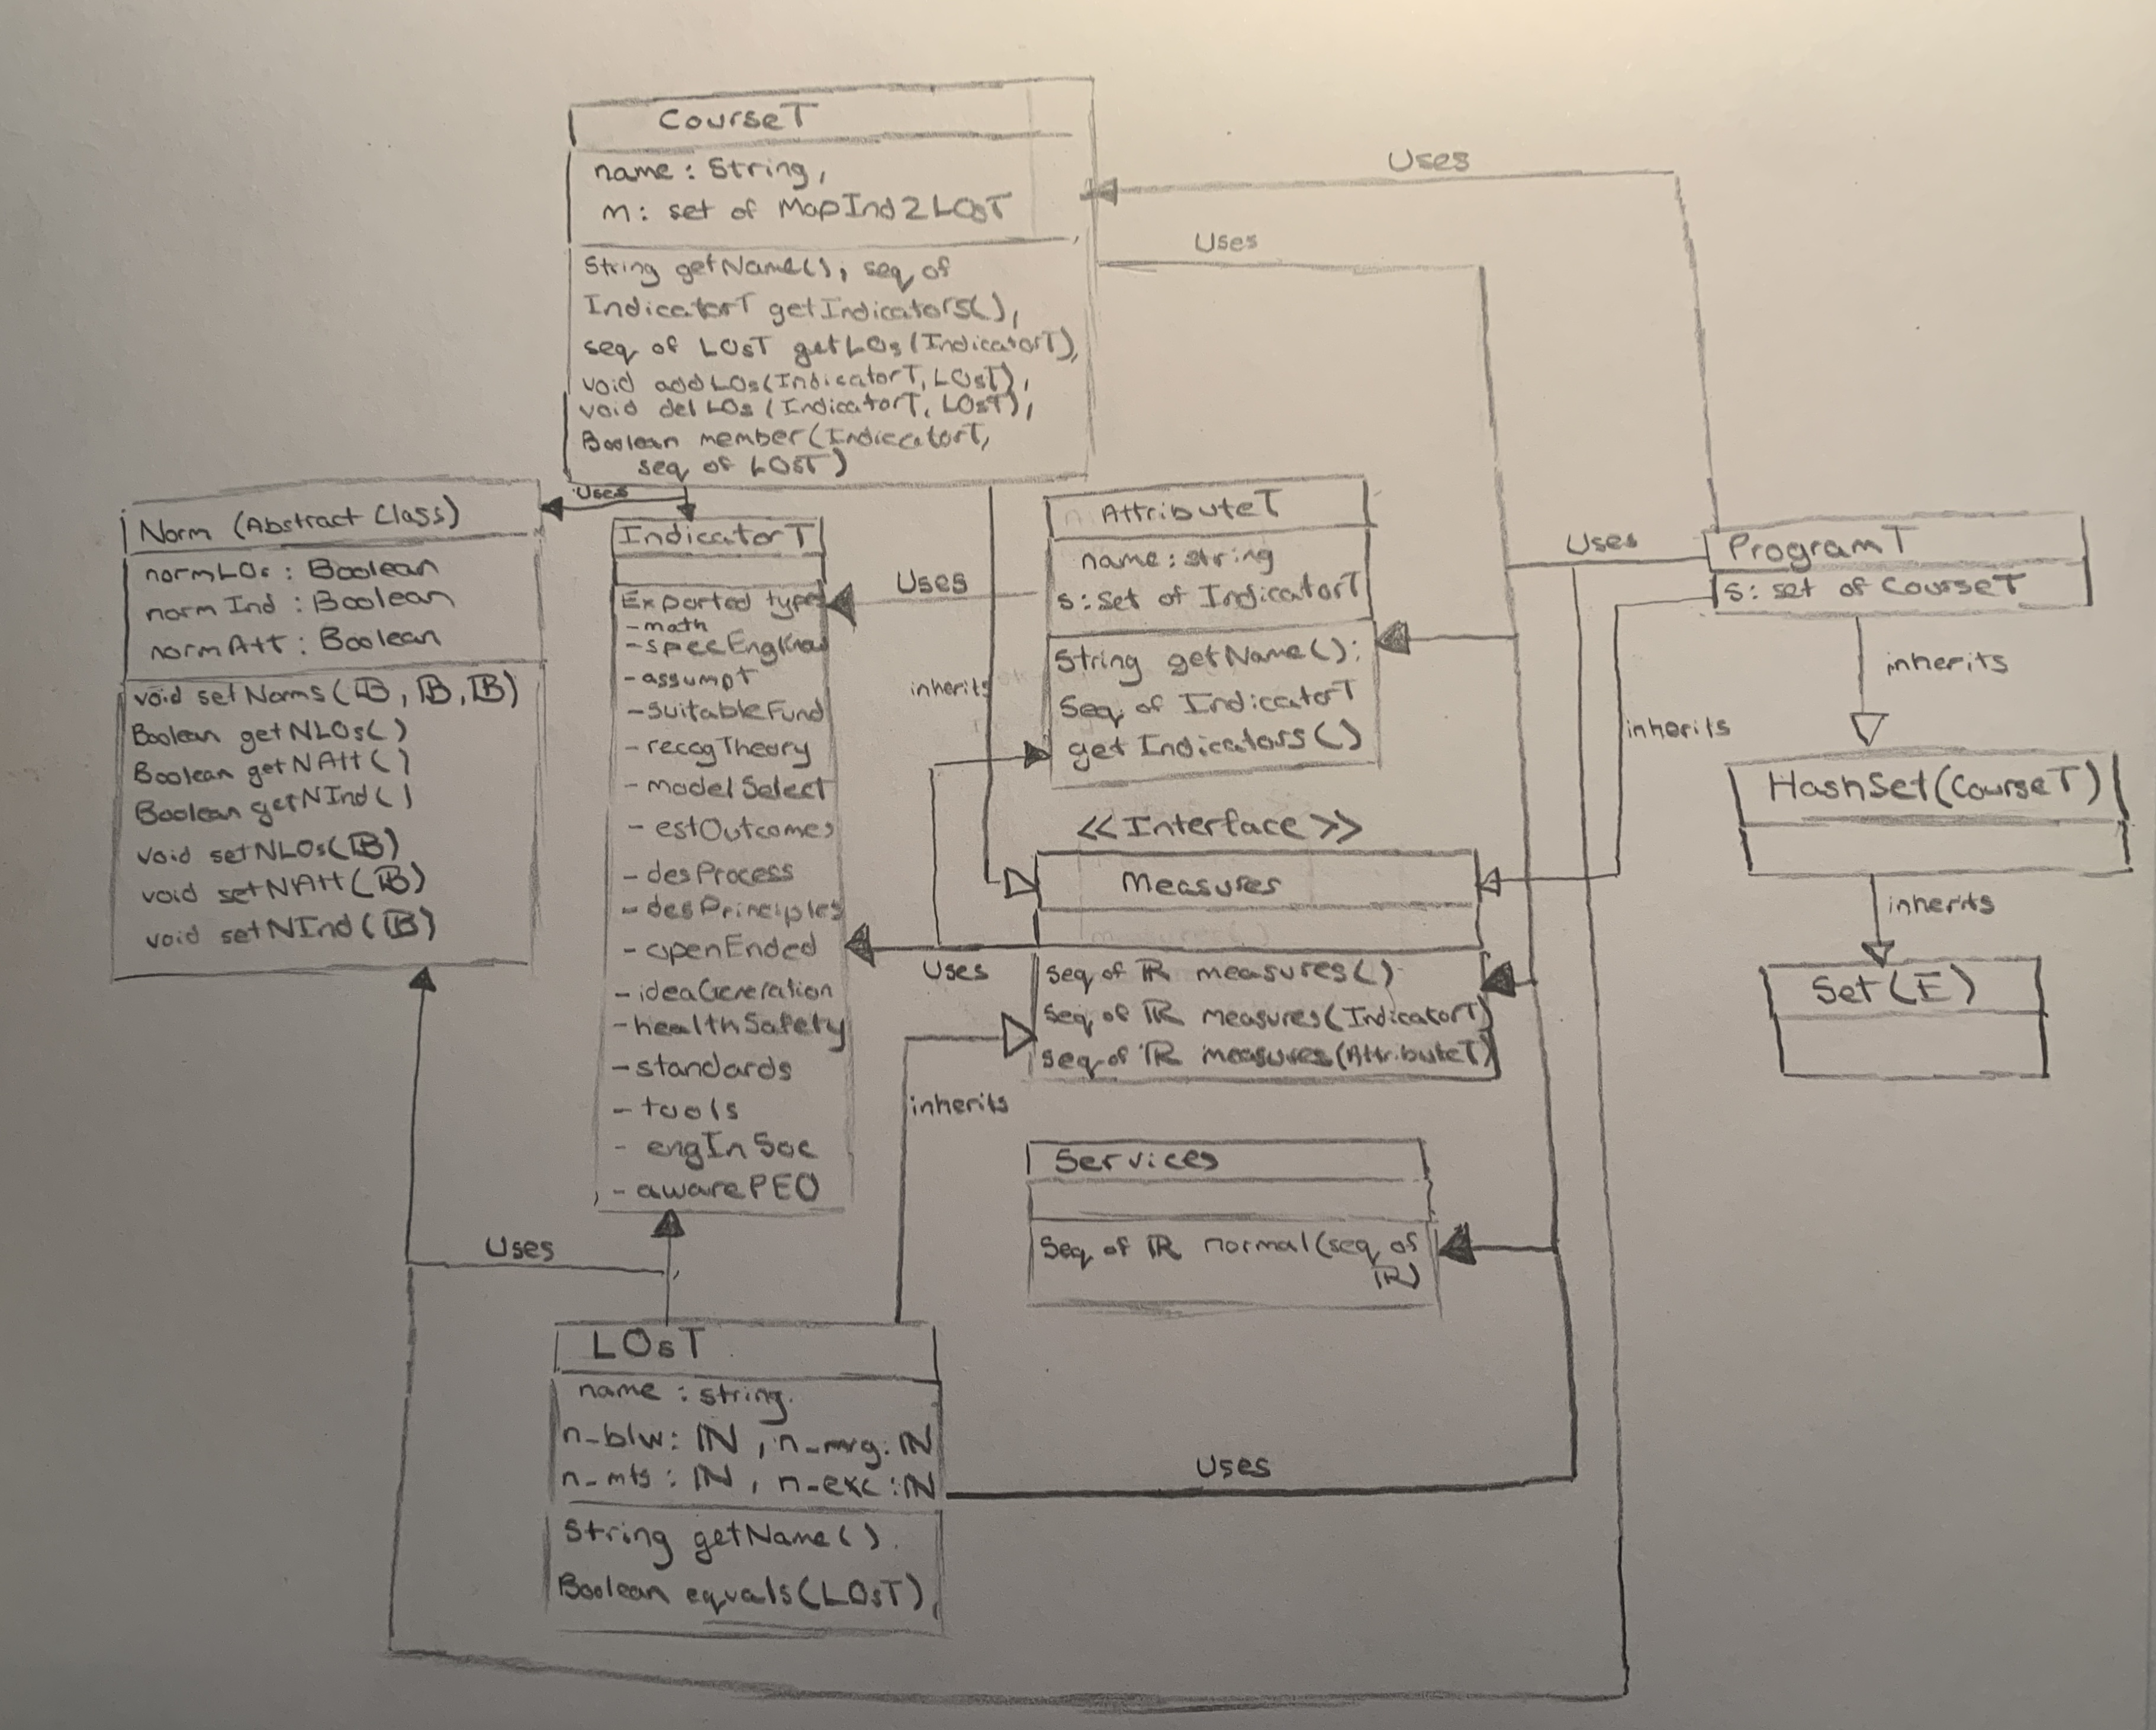
\includegraphics[width=\textwidth,height=\textheight,keepaspectratio]{2me3_A4_Q1.JPG}

\newpage
Q2) Draw a control flow graph for the convex hull algorithm. \\
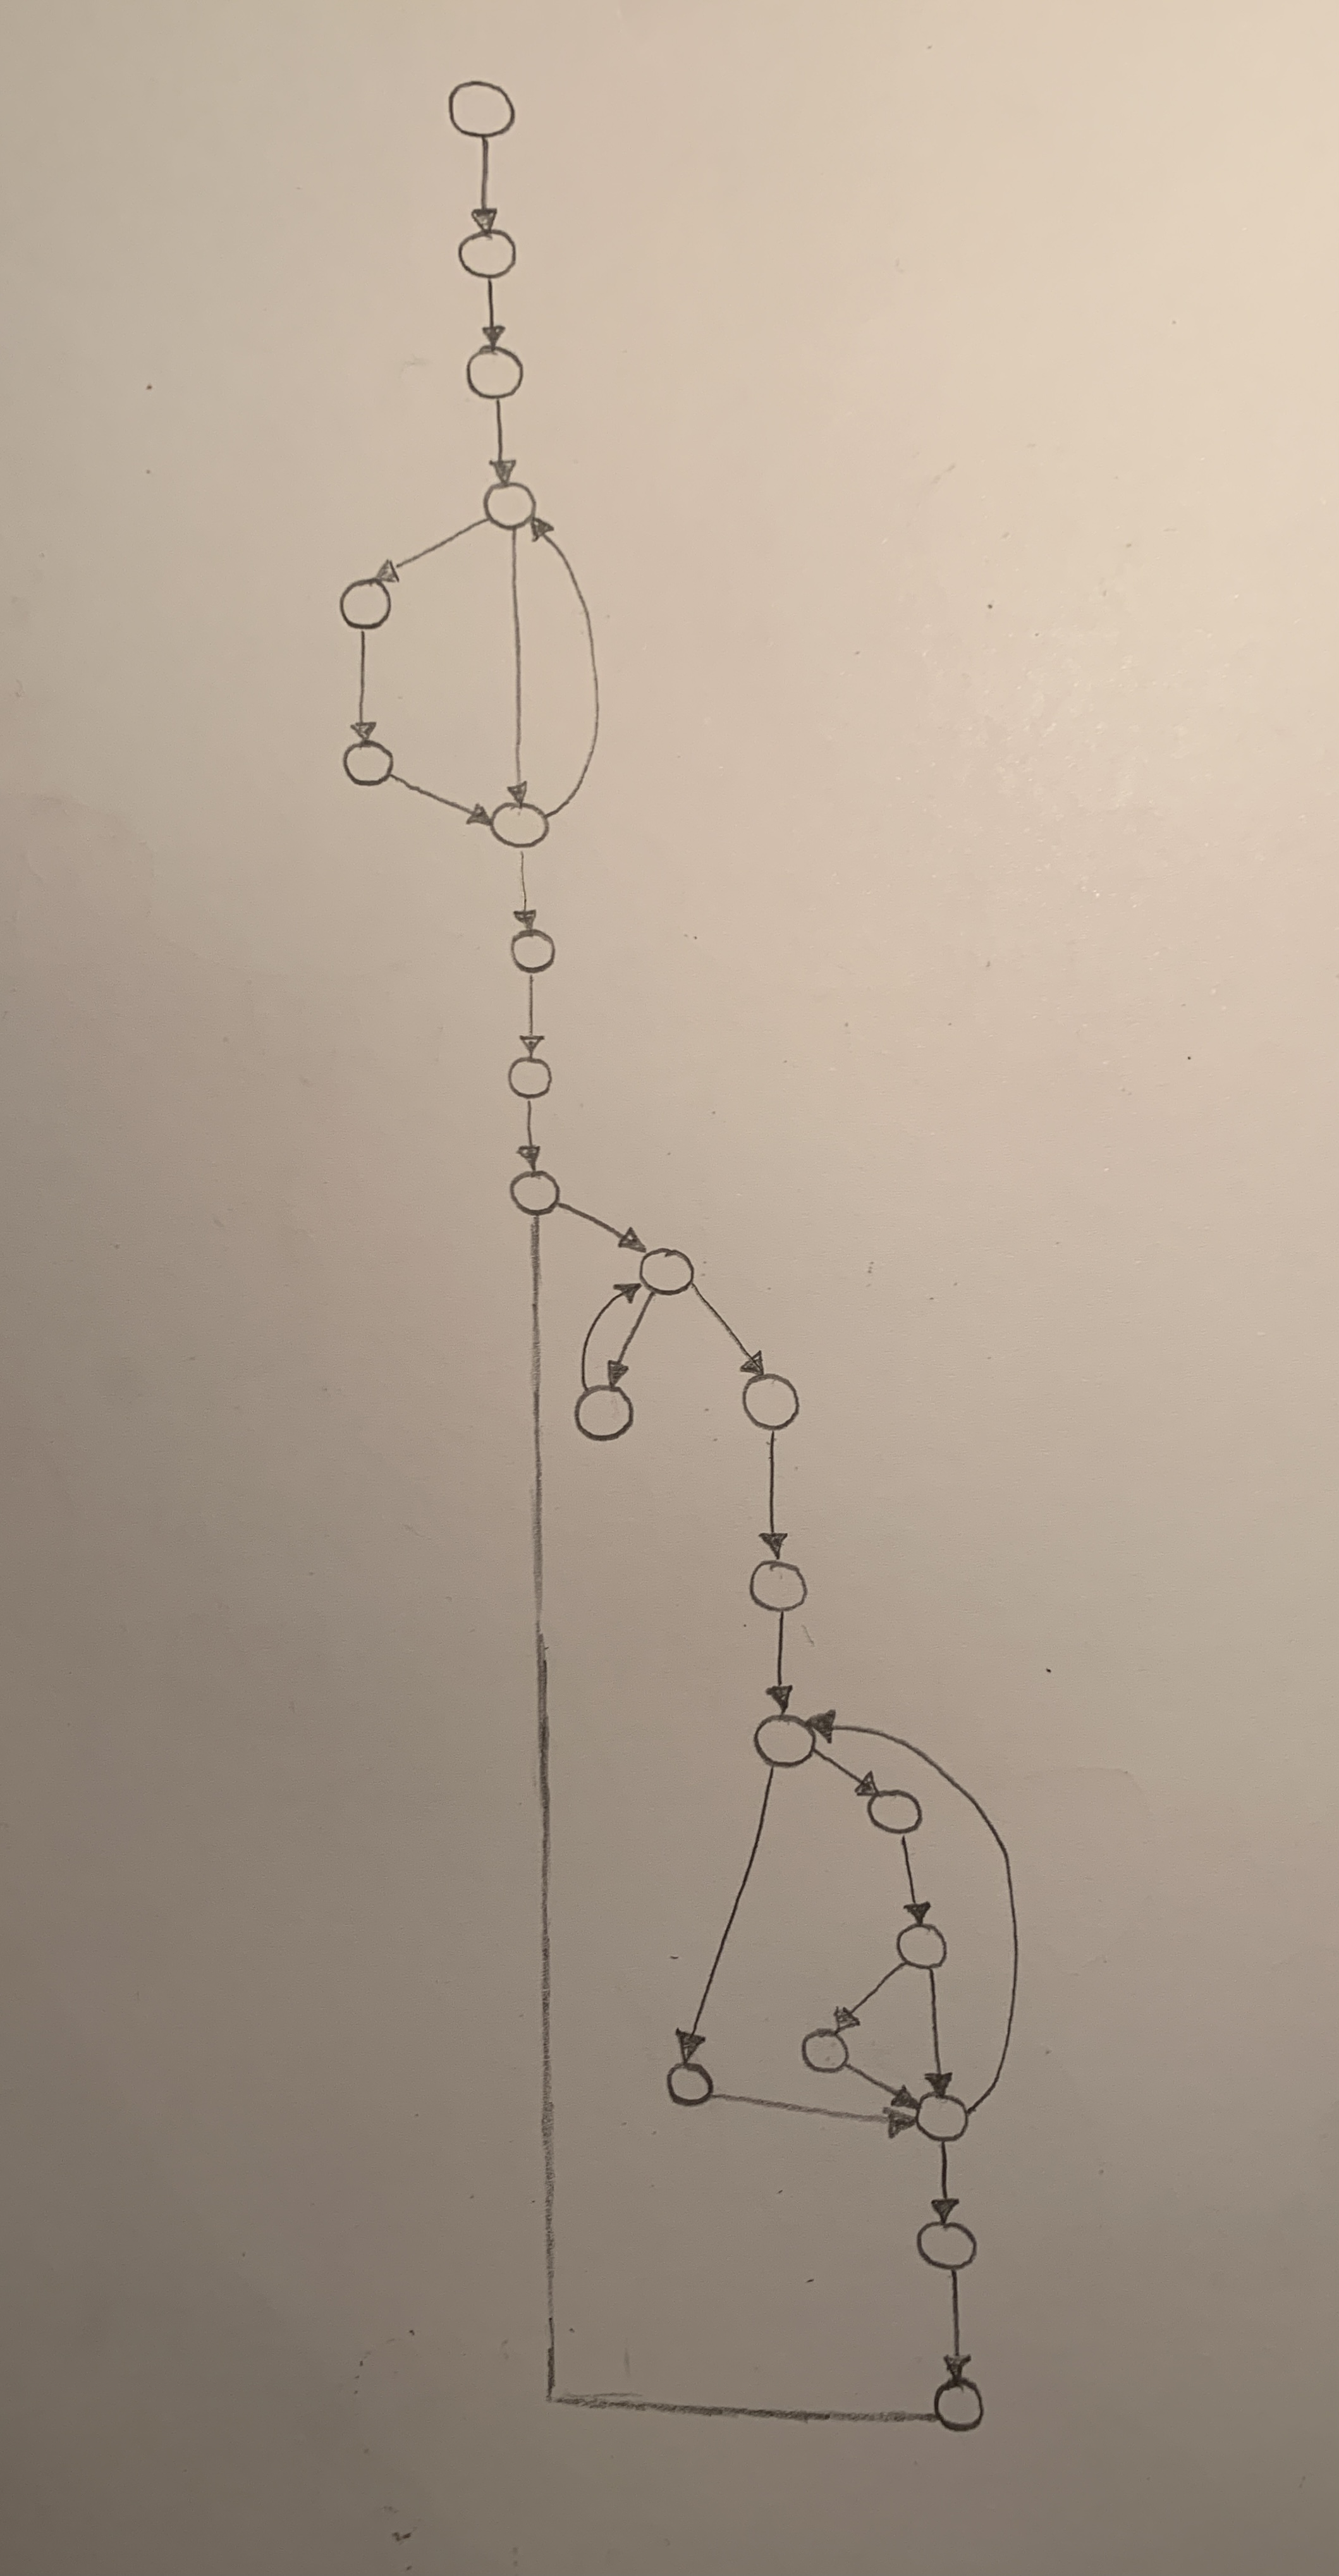
\includegraphics[width=0.9\textwidth,height=0.9\textheight,keepaspectratio]{2me3_A4_Q2.JPG}




\end{document}

